\subsection{Protein Clusters}
Table~\ref{tab:procs} gives the dimensions of the two protein-cluster matrices and how densely they are
filled. Both are sparse, but the viral matrix more so than the bacterial one.

\begin{table}[htbp]
  \centering
  \caption{Protein-cluster matrices, by cohort}
  \label{tab:procs}
  \begin{tabular}{lrrr}
    \hline
                                  &    CRC &    IBD &   GvHD \\
    \hline
    \multicolumn{4}{l}{\textit{Bacteria}} \\
    Genera profiled               &    296 &    285 &    311 \\
    Protein clusters              & 70,625 & 78,517 & 72,646 \\
    Density of $X^{b}$            & 4.38\% & 4.29\% & 4.28\% \\
    Median clusters per genus     &  2,164 &  2,232 &  2,168 \\
    \hline
    \multicolumn{4}{l}{\textit{Viruses}} \\
    vOTUs profiled                &    573 &    692 &    906 \\
    Contigs                       &  6,876 &  8,045 &  5,101 \\
    Median contigs per vOTU       &      3 &      5 &      2 \\
    Protein clusters              &  2,756 &  4,226 &  7,168 \\
    Density of $X^{v}$            & 0.90\% & 0.82\% & 0.76\% \\
    Median clusters per vOTU      &     16 &     20 &     45 \\
    \hline
  \end{tabular}
\end{table}
\FloatBarrier

Figures~\ref{fig:procsparsity-crc} to~\ref{fig:procsparsity-gvhd} show the sparsity of the two
protein-cluster matrices in each cohort.

\begin{figure}[htbp]
  \centering
  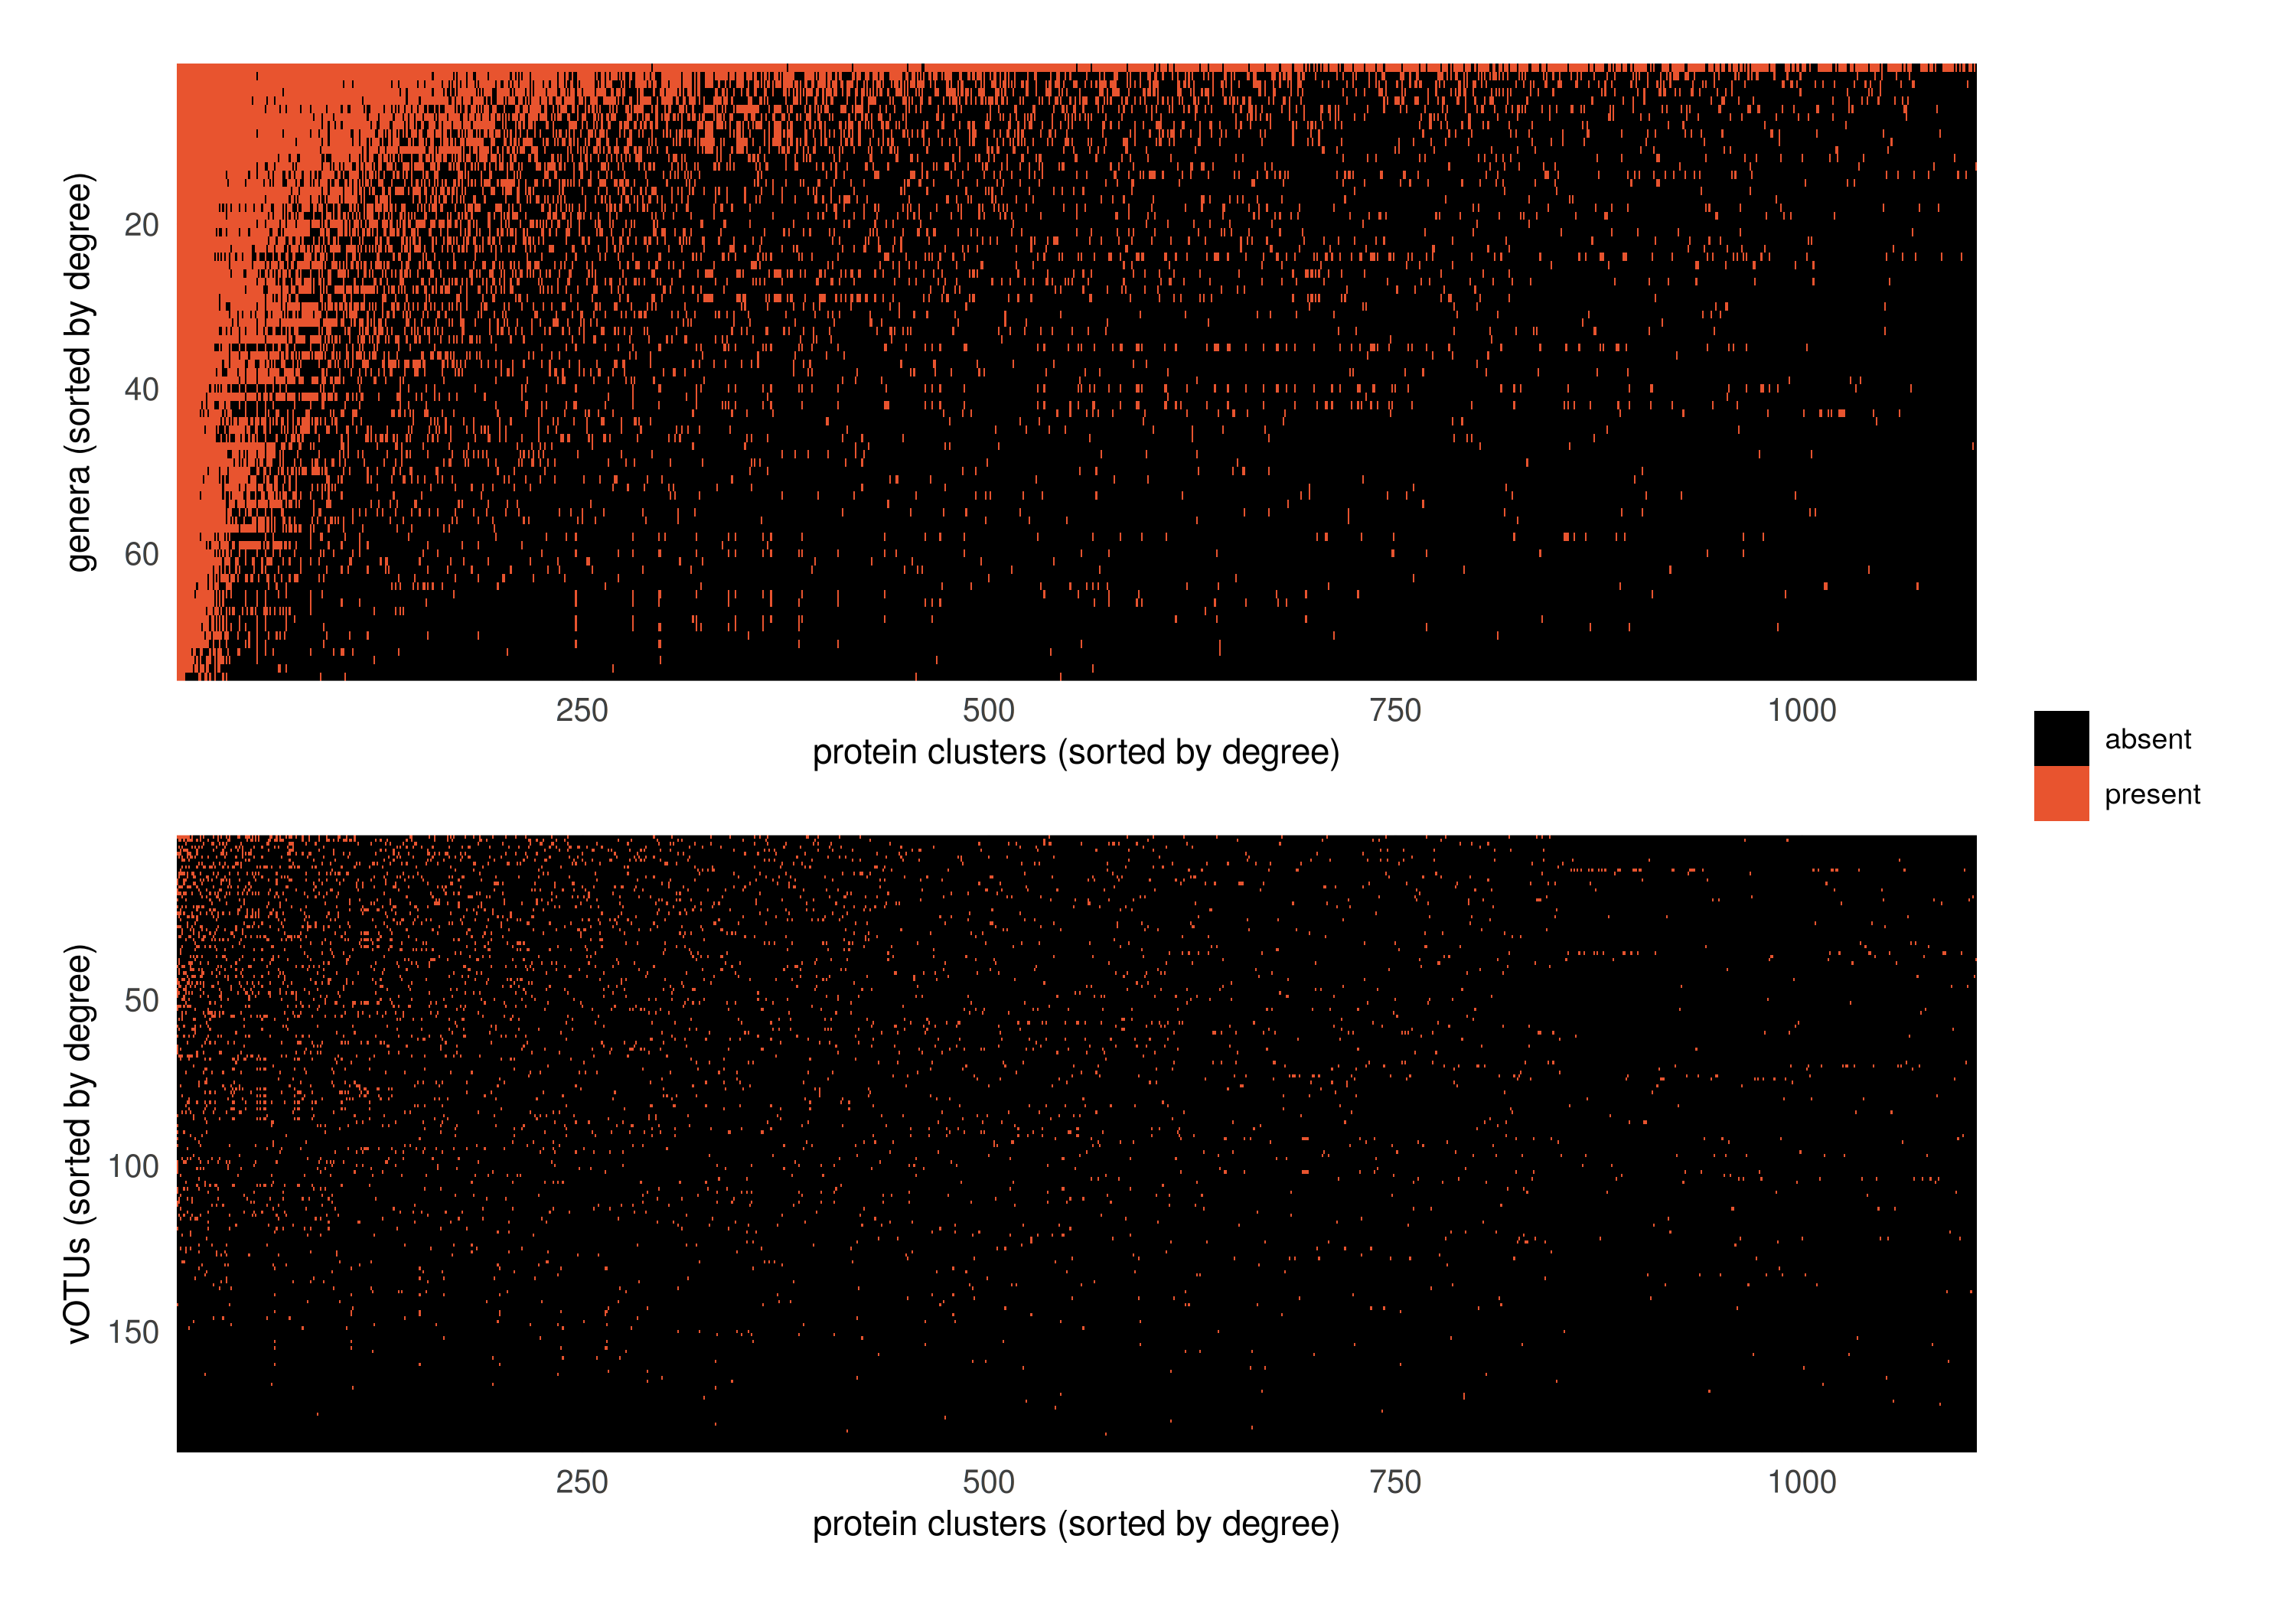
\includegraphics[width=0.88\textwidth]{figures/fig_procsparsity_crc.png}
  \caption{Protein-cluster sparsity, CRC}
  \label{fig:procsparsity-crc}
\end{figure}
\FloatBarrier

\begin{figure}[htbp]
  \centering
  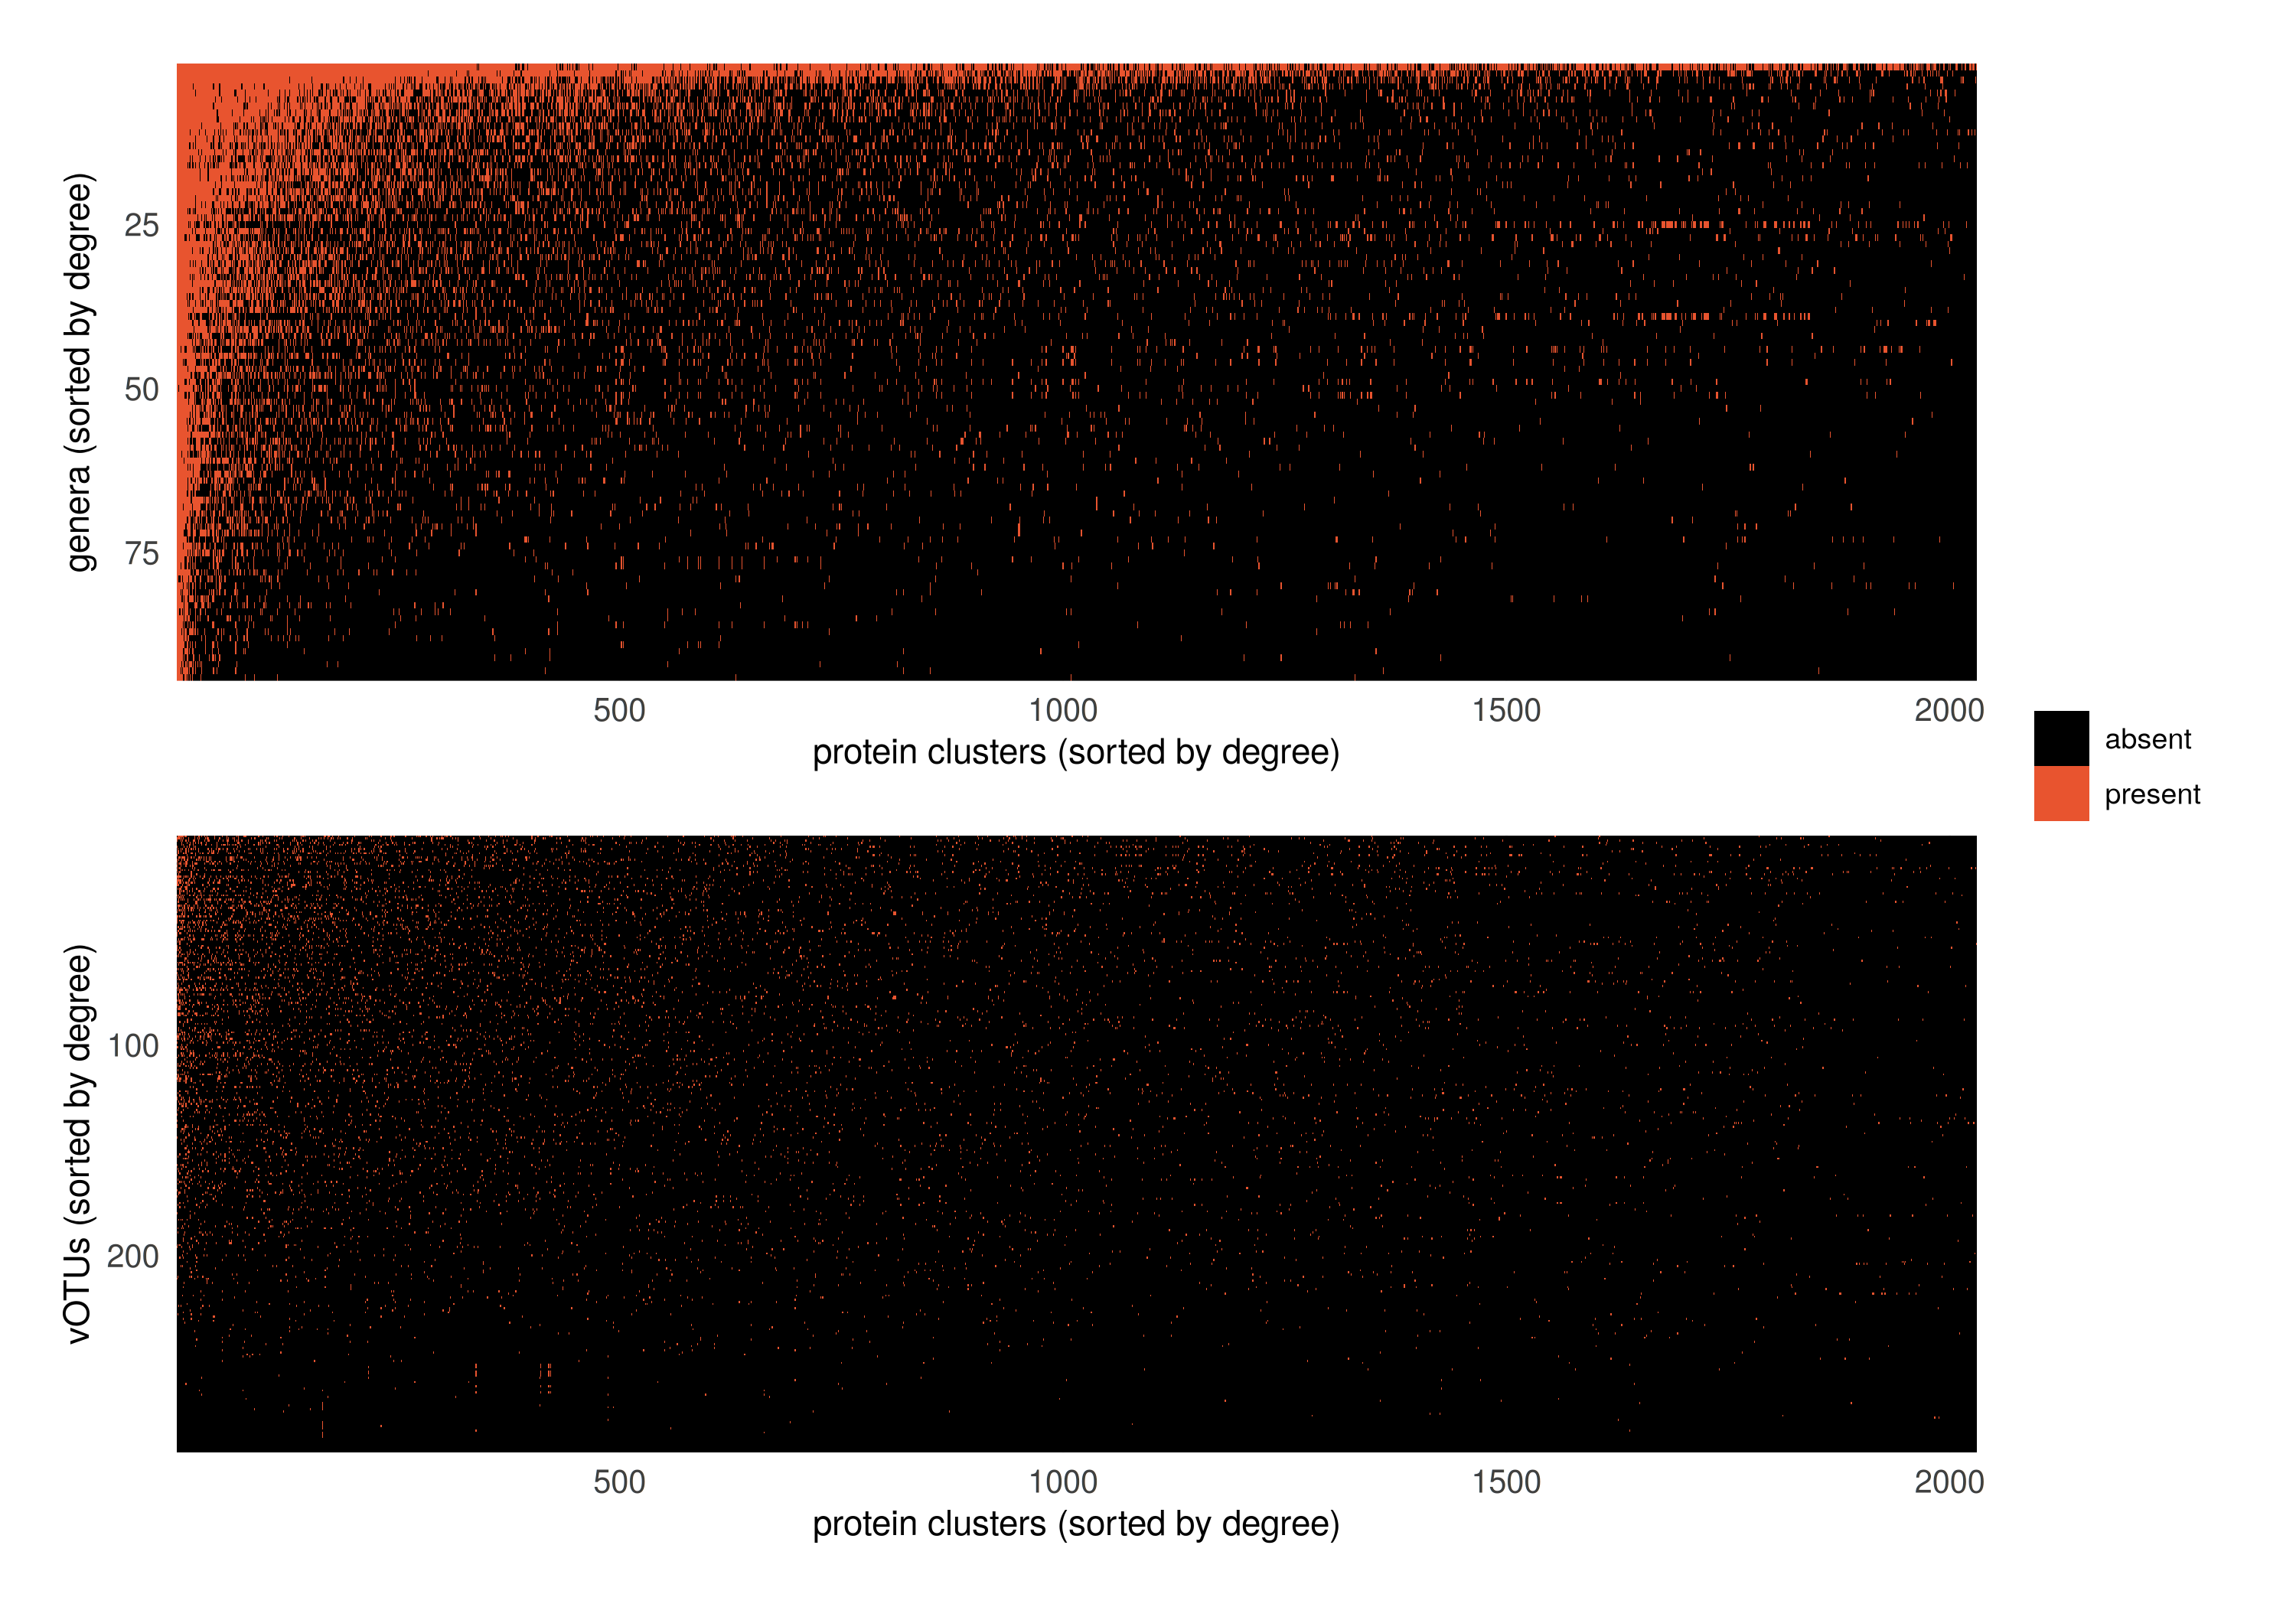
\includegraphics[width=0.88\textwidth]{figures/fig_procsparsity_ibd.png}
  \caption{Protein-cluster sparsity, IBD}
  \label{fig:procsparsity-ibd}
\end{figure}
\FloatBarrier

\begin{figure}[htbp]
  \centering
  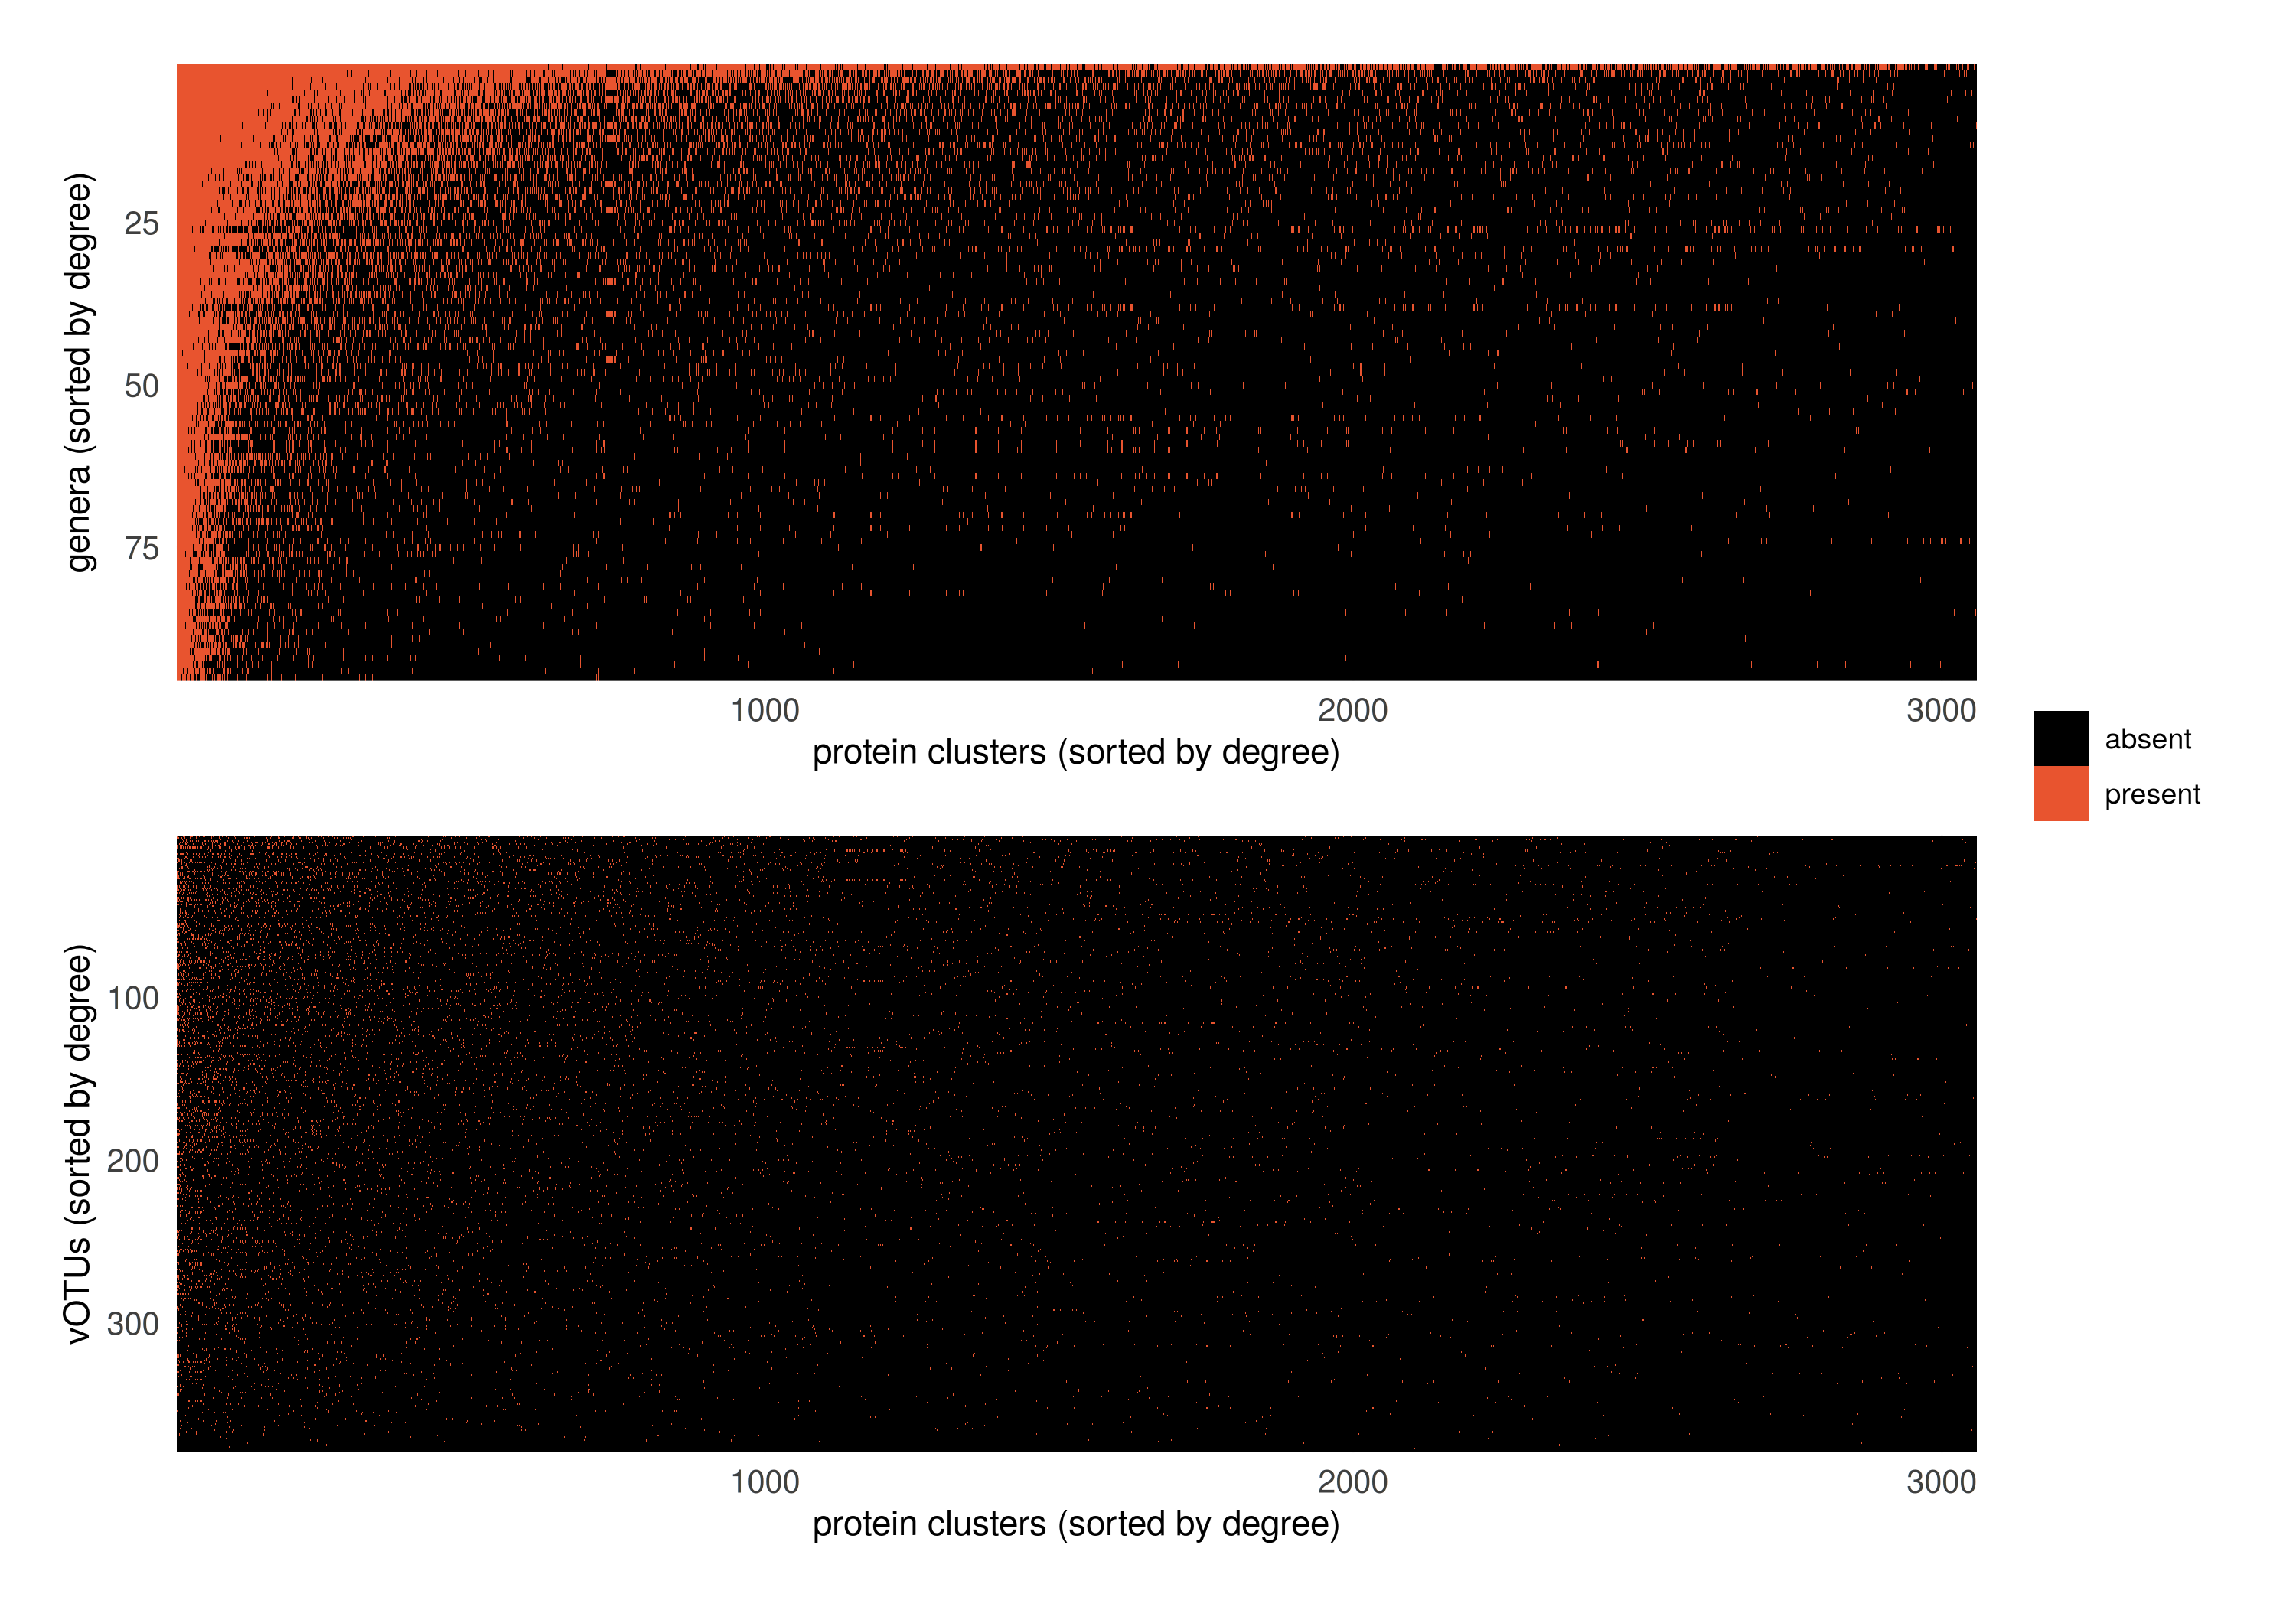
\includegraphics[width=0.88\textwidth]{figures/fig_procsparsity_gvhd.png}
  \caption{Protein-cluster sparsity, GvHD}
  \label{fig:procsparsity-gvhd}
\end{figure}
\FloatBarrier

\subsection{Observed Set of Networks}
\label{res:networks}
Requiring both a protein profile and a CRISPR entry reduces each cohort to the \(n\) bacterial genera and
\(m\) vOTUs that carry both, and the candidate pairs are the \(nm\) combinations of the two. Of the
1{,}360 vOTUs in the CRC viral taxonomy, 573 carry a protein profile and 186 remain once a CRISPR entry
is also required.

The abundance network covers only part of the candidate pairs. In CRC 62 genera and 93 vOTUs are matched,
so the observed set spans 41\% of them; the corresponding figures are $75 \times 70$ (19\%) in IBD and
$56 \times 344$ (54\%) in GvHD. Restricting to the observed pairs barely shifts the CRISPR prevalence,
3.4\% against 3.1\% over all candidate pairs. Table~\ref{tab:descriptives} gives the reduction and both
networks on the observed set.

\begin{table}[htbp]
  \centering
  \caption{Candidate pairs, observed pairs and the two networks, by cohort}
  \label{tab:descriptives}
  \begin{tabular}{lrrr}
    \hline
                              &    CRC &    IBD &   GvHD \\
    \hline
    Samples                   &     84 &    148 &     90 \\
    Bacterial genera kept     &     75 &     94 &     95 \\
    vOTUs kept                &    186 &    293 &    379 \\
    Candidate pairs           & 13,950 & 27,542 & 36,005 \\
    \hline
    Observed pairs            &  5,766 &  5,250 & 19,264 \\
    CRISPR positive           & 198 (3.4\%) & 182 (3.5\%) & 478 (2.5\%) \\
    Selected at least once ($W_{ij}>0$)     & 2,473 (42.9\%) & 2,019 (38.5\%) & 9,451 (49.1\%) \\
    Mean selection probability   &  0.083 &  0.097 &  0.101 \\
    Both                      &     84 &     92 &    265 \\
    \hline
  \end{tabular}
\end{table}
\FloatBarrier

The last row asks whether the two networks mark the same pairs. If they were unrelated, the pairs the
abundance network selects would fall on the observed set without regard to which pairs carry CRISPR
evidence. The overlap is then the number of CRISPR-positive pairs among \(n_W\) draws taken without
replacement from the \(n_{\mathrm{obs}}\) observed pairs, which is hypergeometric. Writing \(n_Y\) and
\(n_W\) for the number of positives of each network,
%
\begin{equation}
  \label{eq:expected-overlap}
  \mathbb{E}[\,\text{both}\,]=\frac{n_Y\,n_W}{n_{\mathrm{obs}}},
  \qquad
  \operatorname{Var}[\,\text{both}\,]
  =n_W\,\frac{n_Y}{n_{\mathrm{obs}}}
   \Bigl(1-\frac{n_Y}{n_{\mathrm{obs}}}\Bigr)
   \frac{n_{\mathrm{obs}}-n_W}{n_{\mathrm{obs}}-1}.
\end{equation}
%
The expected overlap is 85 in CRC, 70 in IBD and 235 in GvHD, against 84, 92 and 265 observed, with
standard deviations of 6.8, 6.4 and 10.8. The observed count is therefore 0.1 standard deviations below
expectation in CRC and 3.4 and 2.8 above it in IBD and GvHD: the two networks mark the same pairs more
often than chance would give in IBD and GvHD, but not in CRC.

In CRC the edge selection probability has a mean of 0.083 and a standard deviation of 0.182, 57\% of the observed
cells are exactly zero and 5\% exceed 0.5. The corresponding shares are 62\% and 7.5\%
in IBD and 51\% and 7.0\% in GvHD.

Over all candidate pairs the median genus carries two to three CRISPR matches and the most connected genus carries 54 in
CRC, 124 in IBD and 156 in GvHD. In every cohort the ten most connected genera account for about 60\% of all
CRISPR edges. The median vOTU carries two matches, with a maximum between 8 and 12.
Figures~\ref{fig:combined-crc} to~\ref{fig:combined-gvhd} show both networks on the observed set: the
edge selection probability as the field and the CRISPR edges outlined on top. Rows and columns are
clustered on \(W\), so the block structure is a property of that ordering.

\begin{figure}[htbp]
  \centering
  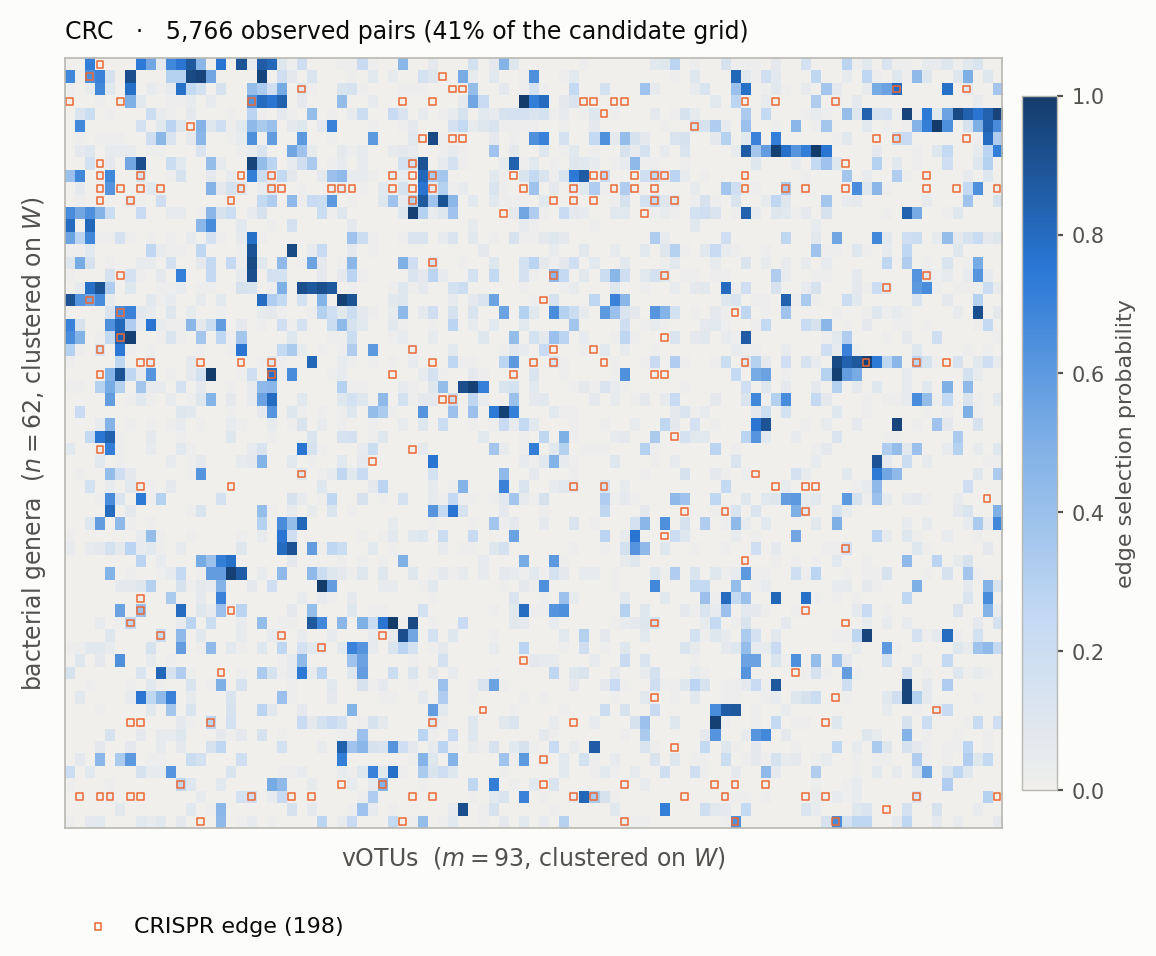
\includegraphics[width=0.80\textwidth]{figures/fig_combined_crc.png}
  \caption{Both networks on the observed set, CRC. Field: edge selection probability. Orange outline: CRISPR edge}
  \label{fig:combined-crc}
\end{figure}
\FloatBarrier

\begin{figure}[htbp]
  \centering
  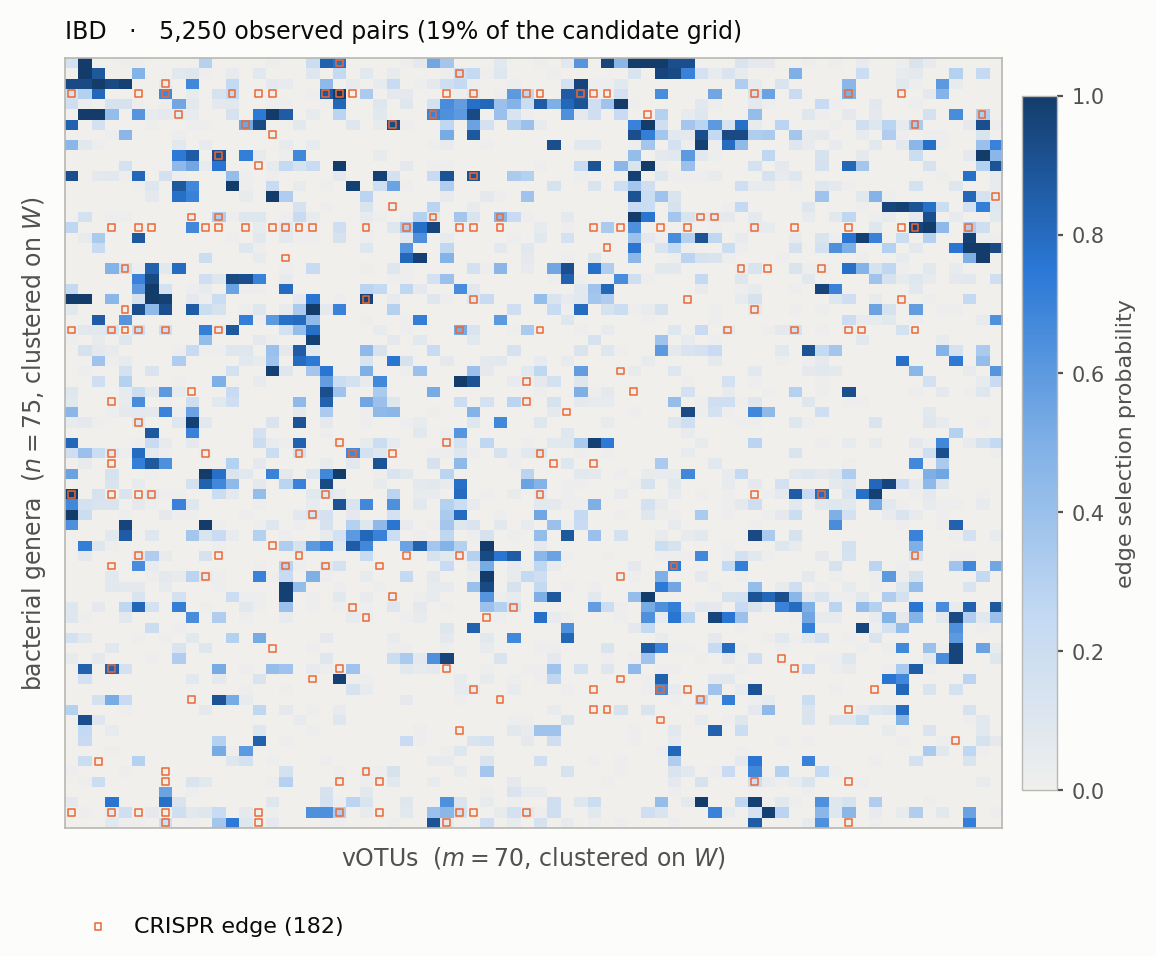
\includegraphics[width=0.80\textwidth]{figures/fig_combined_ibd.png}
  \caption{Both networks on the observed set, IBD. Field: edge selection probability. Orange outline: CRISPR edge}
  \label{fig:combined-ibd}
\end{figure}
\FloatBarrier

\begin{figure}[htbp]
  \centering
  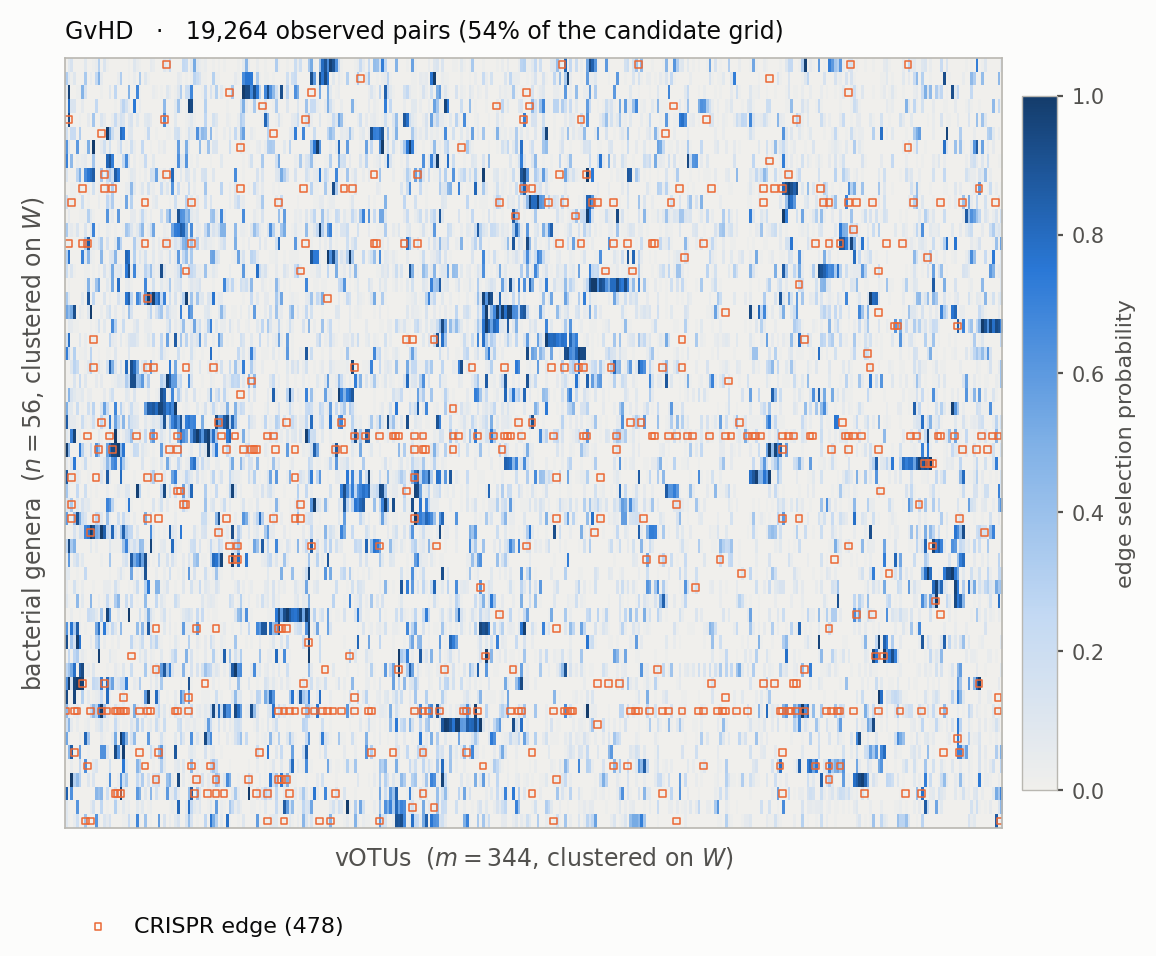
\includegraphics[width=0.80\textwidth]{figures/fig_combined_gvhd.png}
  \caption{Both networks on the observed set, GvHD. Field: edge selection probability. Orange outline: CRISPR edge}
  \label{fig:combined-gvhd}
\end{figure}
\FloatBarrier

\subsection{Prediction Performance}
\label{res:main}

\subsubsection{CRISPR Linkage}
\label{res:main-y}

\begin{table}[htbp]
  \centering
  \caption{Test performance on CRISPR linkage}
  \label{tab:perf-y}
  \begin{tabular}{llrr}
    \hline
    Cohort & Model                     & AUC   & AP    \\
    \hline
    CRC    & Sparse logistic           & 0.758 & 0.185 \\
           & XGBoost                   & 0.788 & 0.213 \\
           & MLP (baseline)            & 0.777 & 0.225 \\
           & MLP (joint)               & 0.775 & 0.253 \\
    \hline
    IBD    & Sparse logistic           & 0.780 & 0.260 \\
           & XGBoost                   & 0.786 & 0.286 \\
           & MLP (baseline)            & 0.740 & 0.269 \\
           & MLP (joint)               & 0.747 & 0.257 \\
    \hline
    GvHD   & Sparse logistic           & 0.767 & 0.129 \\
           & XGBoost                   & 0.798 & 0.186 \\
           & MLP (baseline)            & 0.782 & 0.189 \\
           & MLP (joint)               & 0.780 & 0.200 \\
    \hline
  \end{tabular}
\end{table}

The baseline MLP exceeds sparse logistic on AUC by 0.018 in CRC and 0.015 in GvHD, and is 0.040 below it
in IBD. On AP the difference is $+0.040$ in CRC, $+0.008$ in IBD and $+0.060$ in GvHD.

Against XGBoost the MLP is 0.011 lower in CRC, 0.045 lower in IBD and 0.016 lower in GvHD, whereas on AP
the differences are $+0.012$, $-0.018$ and $+0.003$.

The joint model differs from the baseline MLP on CRISPR AUC by $-0.001$ in CRC, $+0.007$ in IBD and
$-0.001$ in GvHD, with neither model ahead in more than seven of the ten folds. On AP it is 0.028 higher
in CRC, in nine of the ten folds, 0.012 lower in IBD and 0.010 higher in GvHD. The two metrics
therefore disagree in CRC, where sharing a representation leaves the ranking of all pairs unchanged but
improves precision among the highest-scoring ones. At a positive rate of 3.4\% the second is the more
informative comparison, so the joint model is not merely matching the baseline there.

\FloatBarrier

\subsubsection{Edge Selection Probability}
\label{res:main-wreg}

\begin{table}[H]
  \centering
  \caption{Test $R^2$ on the edge selection probability}
  \label{tab:perf-wreg}
  \begin{tabular}{llr}
    \hline
    Cohort & Model              & $R^2$   \\
    \hline
    CRC    & Ridge regression   & $-0.156$ \\
           & XGBoost            & $-0.155$ \\
           & MLP                & $-0.140$ \\
    \hline
    IBD    & Ridge regression   & $-0.153$ \\
           & XGBoost            & $-0.161$ \\
           & MLP                & $-0.130$ \\
    \hline
    GvHD   & Ridge regression   & $-0.172$ \\
           & XGBoost            & $-0.179$ \\
           & MLP                & $-0.143$ \\
    \hline
  \end{tabular}
\end{table}

$R^2$ is negative for every model in every cohort, ranging from $-0.130$ to $-0.179$, and no individual fold of
any model reaches zero.

\subsubsection{Binarised Selection Probability}
\label{res:main-wclass}

\begin{table}[htbp]
  \centering
  \caption{Test performance on the binarised selection probability}
  \label{tab:perf-wclass}
  \begin{tabular}{llrr}
    \hline
    Cohort & Model                     & AUC   & AP    \\
    \hline
    CRC    & Sparse logistic           & 0.590 & 0.498 \\
           & XGBoost                   & 0.579 & 0.495 \\
           & MLP (baseline)            & 0.567 & 0.485 \\
           & MLP (joint)               & 0.586 & 0.501 \\
    \hline
    IBD    & Sparse logistic           & 0.578 & 0.442 \\
           & XGBoost                   & 0.578 & 0.455 \\
           & MLP (baseline)            & 0.606 & 0.480 \\
           & MLP (joint)               & 0.605 & 0.480 \\
    \hline
    GvHD   & Sparse logistic           & 0.599 & 0.582 \\
           & XGBoost                   & 0.590 & 0.568 \\
           & MLP (baseline)            & 0.590 & 0.570 \\
           & MLP (joint)               & 0.603 & 0.586 \\
    \hline
  \end{tabular}
\end{table}

Every model in every cohort sits between 0.567 and 0.606 AUC. The baseline MLP is 0.023 below sparse
logistic in CRC, 0.028 above it in IBD and 0.008 below it in GvHD; on AP the differences are $-0.013$,
$+0.038$ and $-0.012$. XGBoost is 0.011 below sparse logistic in CRC, level with it in IBD and 0.009 below
in GvHD.

The joint model exceeds the baseline MLP by 0.020 in CRC and 0.013 in GvHD, in nine and eight of the ten
folds, with a difference of $-0.001$ in IBD. Against sparse logistic it is 0.004 lower in CRC, 0.027
higher in IBD and 0.004 higher in GvHD.

\FloatBarrier

\subsection{Representation Comparison}
\label{res:cka}
We compute all values below on latent coordinates scaled to unit variance and report them as a mean and
standard deviation over the ten held-out folds.

The two single-head layers are the least aligned pair in every cohort, at 0.264 (0.010) in CRC,
0.134 (0.019) in IBD and 0.093 (0.024) in GvHD. The shared layer of the joint model is far closer to the
layer fitted to \(Y\), at 0.768 (0.016), 0.565 (0.049) and 0.847 (0.041), than to the layer fitted to the
binarised edge weight, at 0.345 (0.019), 0.386 (0.015) and 0.167 (0.024).

The alignment of the shared layer with the layer fitted to the binarised edge weight nevertheless
exceeds that between the two single-head layers in all three cohorts, by 0.081 in CRC, 0.251 in IBD
and 0.073 in GvHD.

Fold-to-fold variation is small, between 0.010 and 0.024 for seven of the nine values; the exceptions are
the alignment with \(H^{Y}\) in IBD (0.049) and in GvHD (0.041).
Figures~\ref{fig:cka-crc} to~\ref{fig:cka-gvhd} show the three pairwise values per cohort.

\begin{figure}[htbp]
  \centering
  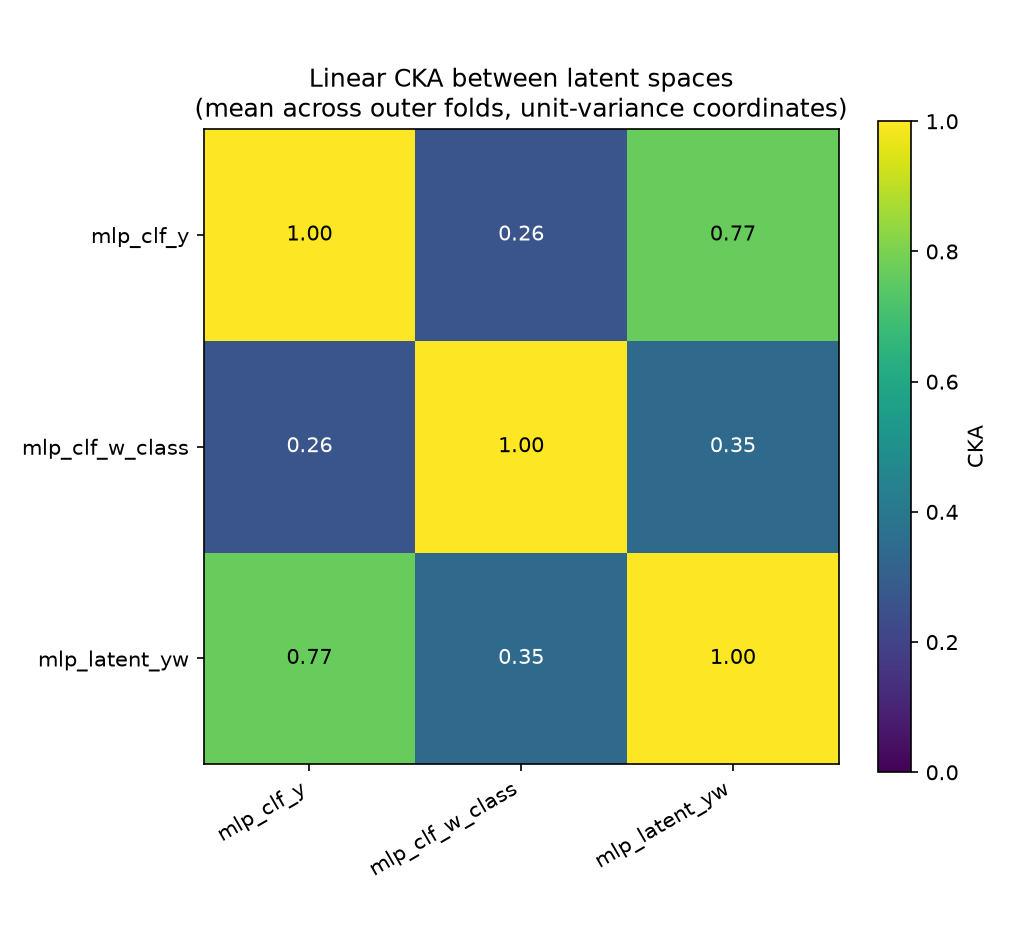
\includegraphics[width=0.60\textwidth]{figures/fig_cka_crc.png}
  \caption{Linear CKA between the fitted hidden layers on unit-variance coordinates, mean over the ten
  held-out folds, CRC}
  \label{fig:cka-crc}
\end{figure}
\FloatBarrier

\begin{figure}[htbp]
  \centering
  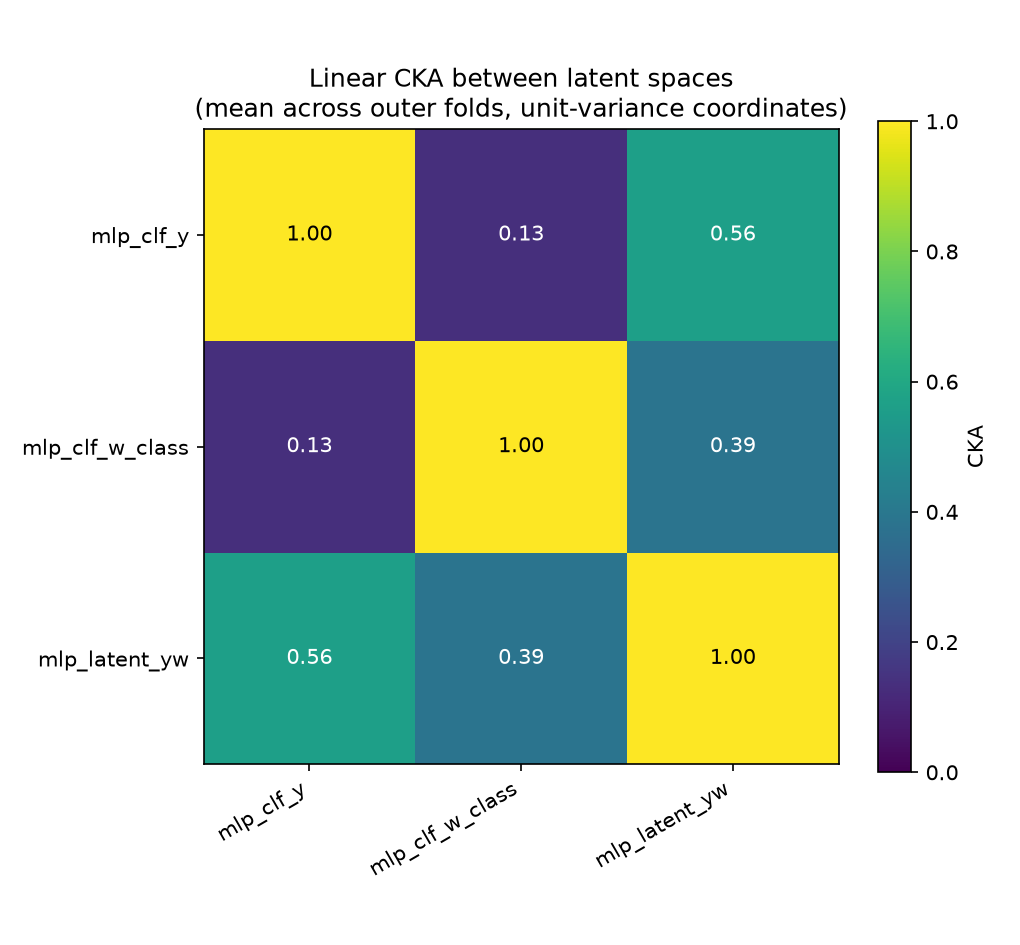
\includegraphics[width=0.60\textwidth]{figures/fig_cka_ibd.png}
  \caption{Linear CKA between the fitted hidden layers on unit-variance coordinates, mean over the ten
  held-out folds, IBD}
  \label{fig:cka-ibd}
\end{figure}
\FloatBarrier

\begin{figure}[htbp]
  \centering
  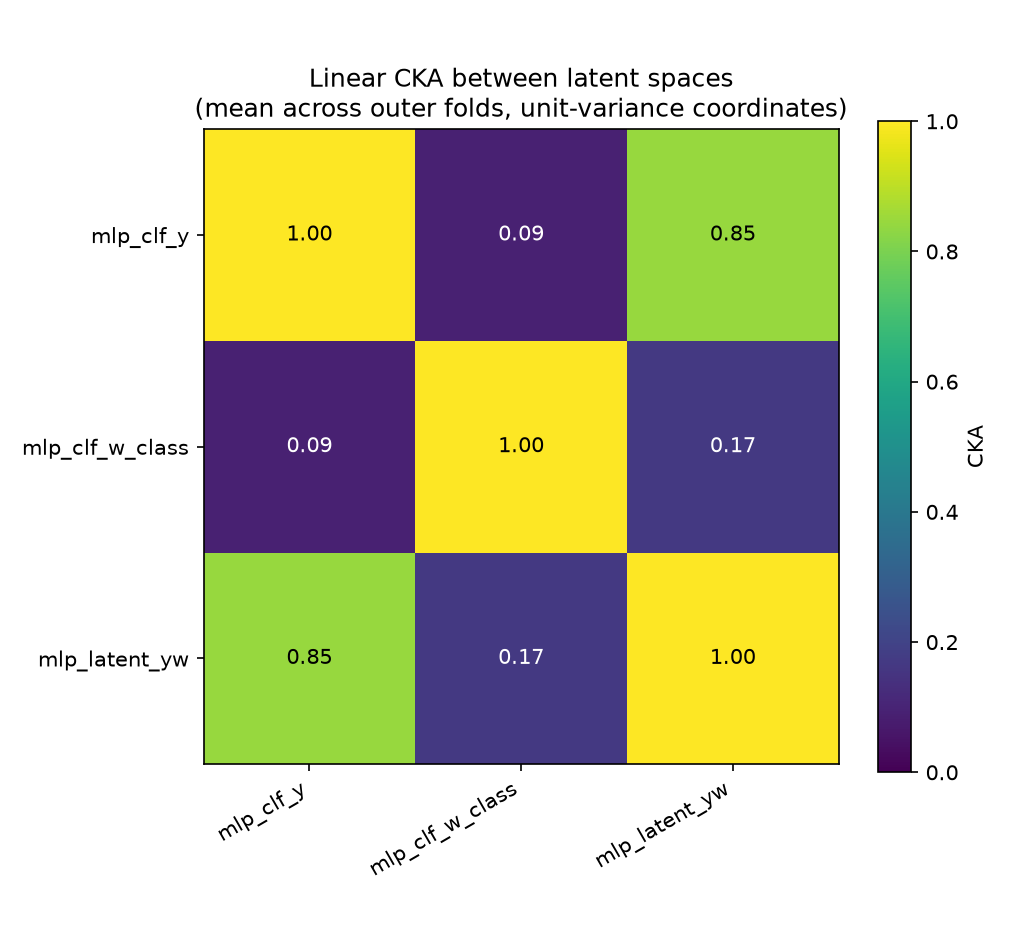
\includegraphics[width=0.60\textwidth]{figures/fig_cka_gvhd.png}
  \caption{Linear CKA between the fitted hidden layers on unit-variance coordinates, mean over the ten
  held-out folds, GvHD}
  \label{fig:cka-gvhd}
\end{figure}
\FloatBarrier

\subsection{Shuffled-CRISPR Control}
\label{res:joint}

\begin{table}[htbp]
  \centering
  \caption{Shuffled-CRISPR control: real vs permuted CRISPR labels}
  \label{tab:shuffle-y}
  \begin{tabular}{lllrr}
    \hline
    Cohort & Head               & CRISPR labels & AUC   & AP    \\
    \hline
    CRC    & CRISPR             & Real       & 0.775 & 0.253 \\
           &                    & Permuted   & 0.476 & 0.042 \\
           & edge selection probability        & Real       & 0.586 & 0.501 \\
           &                    & Permuted   & 0.580 & 0.496 \\
    \hline
    IBD    & CRISPR             & Real       & 0.747 & 0.257 \\
           &                    & Permuted   & 0.487 & 0.050 \\
           & edge selection probability        & Real       & 0.605 & 0.480 \\
           &                    & Permuted   & 0.599 & 0.475 \\
    \hline
    GvHD   & CRISPR             & Real       & 0.780 & 0.200 \\
           &                    & Permuted   & 0.508 & 0.031 \\
           & edge selection probability        & Real       & 0.603 & 0.586 \\
           &                    & Permuted   & 0.602 & 0.587 \\
    \hline
  \end{tabular}
\end{table}

On the CRISPR head the permutation moves AUC from 0.747--0.780 to 0.476--0.508 and AP from 0.200--0.257
to 0.031--0.050, in every fold of every cohort.

On the association head the difference between real and permuted CRISPR labels is $+0.007$ in CRC,
$+0.005$ in IBD and $+0.001$ in GvHD, with the real labels ahead on AUC in eight, seven and six of the ten
folds. The permuted joint model reaches 0.580 on the edge selection probability against 0.567 for the baseline
 MLP in CRC, 0.599 against 0.606 in IBD and 0.602 against 0.590 in GvHD.

Figures~\ref{fig:shuffle-crc} to~\ref{fig:shuffle-gvhd} give the real and permuted scores per cohort.

\begin{figure}[htbp]
  \centering
  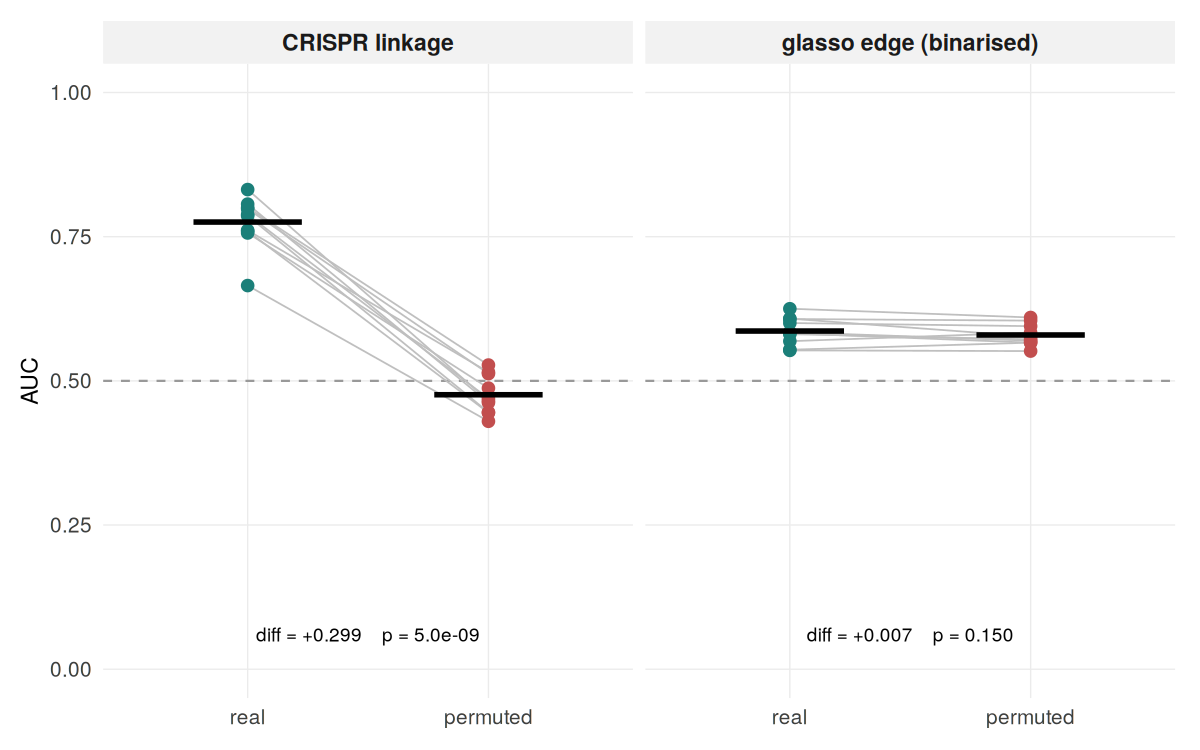
\includegraphics[width=0.88\textwidth]{figures/fig_shuffle_crc.png}
  \caption{Real against permuted CRISPR labels, CRC}
  \label{fig:shuffle-crc}
\end{figure}
\FloatBarrier

\begin{figure}[htbp]
  \centering
  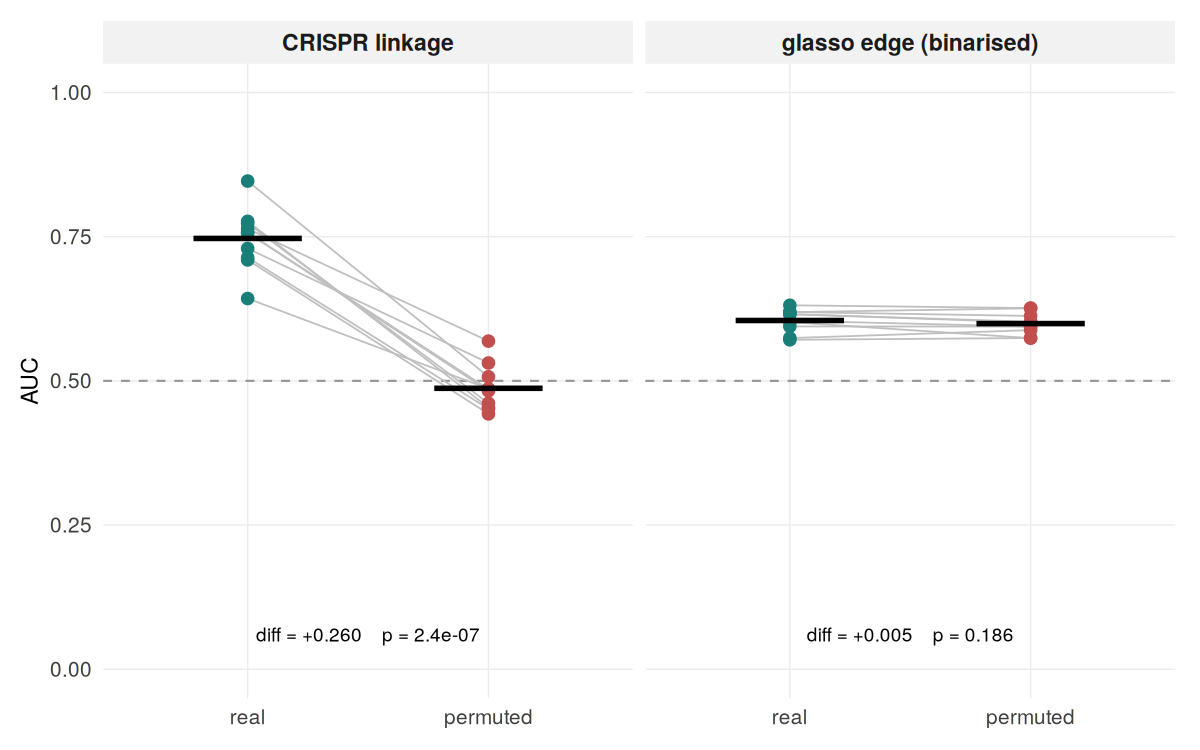
\includegraphics[width=0.88\textwidth]{figures/fig_shuffle_ibd.png}
  \caption{Real against permuted CRISPR labels, IBD}
  \label{fig:shuffle-ibd}
\end{figure}
\FloatBarrier

\begin{figure}[htbp]
  \centering
  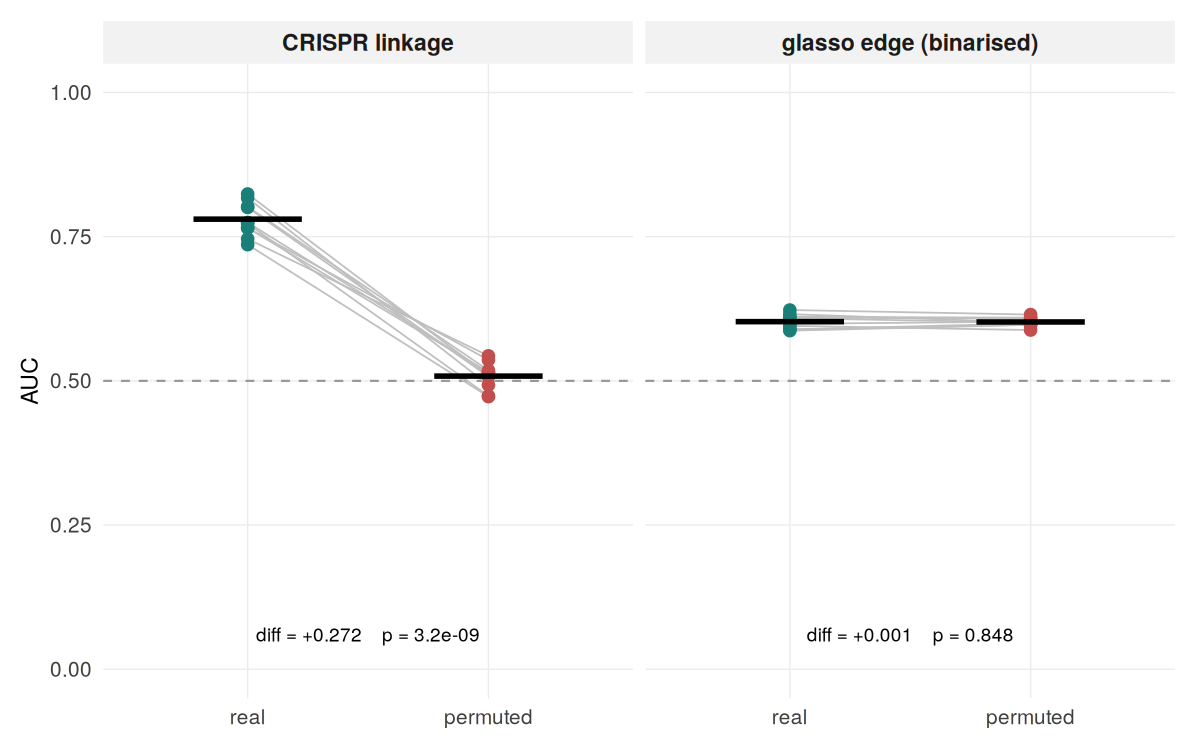
\includegraphics[width=0.88\textwidth]{figures/fig_shuffle_gvhd.png}
  \caption{Real against permuted CRISPR labels, GvHD}
  \label{fig:shuffle-gvhd}
\end{figure}
\FloatBarrier
\subsection{Stability Selection}
\label{res:stability}
Table~\ref{tab:stability} gives the stability selection over the shared protein clusters, run on CRISPR linkage
over the observed pairs with $B = 50$ subsamples at $\pi_{\mathrm{thr}} = 0.8$. The candidate set is 1{,}103
clusters in CRC, 2{,}013 in IBD and 3{,}051 in GvHD, giving $q = 25$, $34$ and $42$. Every resample reached
$q$, with an average support of 27.5, 36.8 and 47.2 clusters, so the bound of
Equation~\eqref{eq:mbbound} evaluated at the realised average support is 1.14, 1.12 and 1.21.

No cluster reaches the threshold in any cohort, and none is selected in half of the resamples. The highest
selection probability is 0.46 in CRC, 0.36 in IBD and 0.30 in GvHD.
Figure~\ref{fig:ap-stab} in the appendix gives the selection probabilities per cohort.

\begin{table}[htbp]
  \centering
  \caption{Stability selection over the shared protein clusters, CRISPR linkage}
  \label{tab:stability}
  \begin{tabular}{lrrrrrr}
    \hline
    Cohort & $n_{\text{obs}}$ & $d$ & $q$ & Mean support & Stable & Max.\ selection prob. \\
    \hline
    CRC  &  5,766 & 1,103 & 25 & 27.5 & 0 & 0.46 \\
    IBD  &  5,250 & 2,013 & 34 & 36.8 & 0 & 0.36 \\
    GvHD & 19,264 & 3,051 & 42 & 47.2 & 0 & 0.30 \\
    \hline
  \end{tabular}
\end{table}
\FloatBarrier

